\documentclass{article}
\usepackage{xeCJK}
\usepackage[margin = 0.75cm, a4paper]{geometry}
\setCJKmainfont{Noto Serif CJK TC}
\setCJKsansfont{Noto Sans CJK TC}
\setCJKmonofont{Noto Sans Mono CJK TC}
\usepackage{booktabs}
\usepackage{float}
\usepackage{graphicx}
\begin{document}
\begin{center}
    \Large Trustworthy AI HW 2\\
    \Large R15922098 李冠誼
\end{center}
\section{Experiment 1 - Implement Memory Mechanism}
\subsection{Architecture}
Figure~\ref{fig:memory} shows the final memory mechanism, which was built step by step in Update 1--4.
\textbf{Write}: \texttt{chat()} stores every utterance except questions to the agent, and tags statements whose subject is another person (Update 2, 4).
\textbf{Read}: \texttt{prepare()} computes arithmetic questions in Python (Update 1); otherwise it scores the sentences about the user by bigram overlap and topic words, and returns the matched sentences within 300 characters (Update 2--4).
\textbf{Update}: a repeated sentence keeps only its latest copy, arithmetic uses the latest value, and the returned sentences are sorted by time, so the newest value is always the later line.
\textbf{Abstention}: if no sentence matches, \texttt{prepare()} returns an empty context, which leads the model to choose 你沒有提過.
\begin{figure}[H]
    \centering
    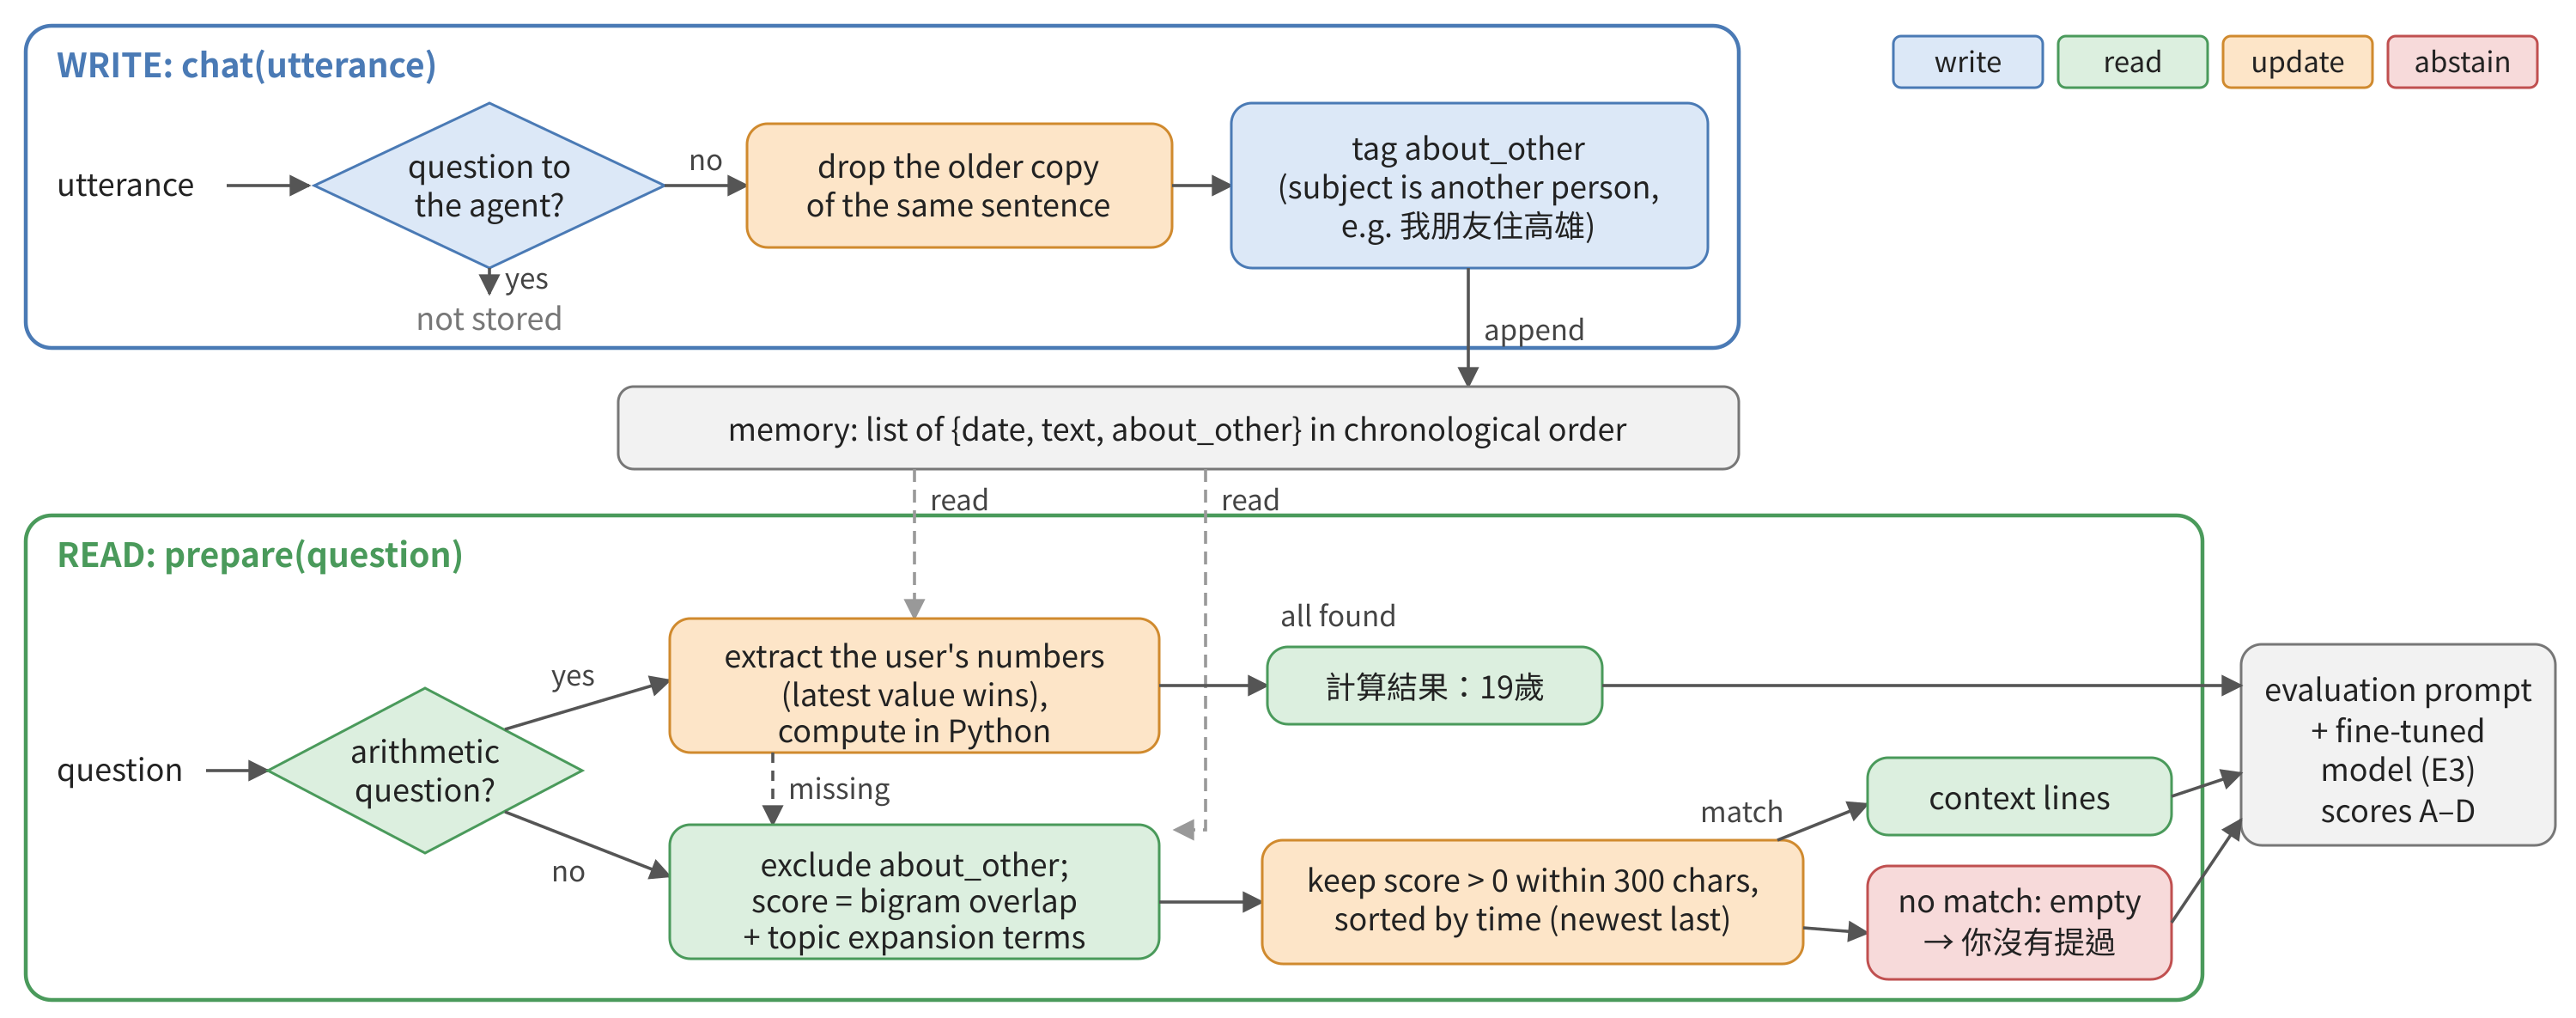
\includegraphics[width=0.85\linewidth]{memory_diagram.png}
    \caption{Memory mechanism of the agent. Colors mark the four memory operations.}
    \label{fig:memory}
\end{figure}
\subsection{Update 1 - Solve Calculation Problem by Direct Computation}
\subsubsection{Motivation}
In the \texttt{KeywordRetrievalAgent}, the tool questions reached only 0.30 accuracy. There are two assumed reasons.
First, \texttt{prepare()} often failed to find the needed facts. 
Second, even when it found them, the 64M model may not be able to do the arithmetic.
To fix these two problems, solving calculation problem by direct computation is a method worthy to try.
\subsubsection{Solution}
\texttt{prepare()} was modified. The new \texttt{prepare()} checks whether a question needs calculation by rule-based function at first.
Then, it looks up the relevant numbers the user mentioned, computes the answer in Python and returns only the result. (e.g., 計算結果: 19歲)
On Table~\ref{tab:diff}, tool-type accuracy rose from 0.30 to 0.98, so Mem Acc rose by 0.114 and LB by 0.080.
\subsection{Update 2 - Avoid Saving Small Talk and Interrogative Sentences}
\subsubsection{Motivation}
We observed that 61-83\% of the lines retrieved by \texttt{prepare()} were small talk, and the same sentence was often repeated several times. 
The interrogative words in the question may match unrelated sentences.
For example, 我叫什麼名字? retrieved 你覺得周末做什麼好? only because both contain 什麼.
Besides, small talk repeats: on average 68 of the 128 utterances of a persona are duplicates.
\subsubsection{Solution}
\texttt{chat()} was modified to skip utterances that are entirely questions to the agent and to keep only the latest copy of a repeated sentence.
In \texttt{prepare()}, interrogative and function words (e.g., 什麼, 哪, 嗎) are removed from the question before matching.
On Table~\ref{tab:diff}, single rose by 0.02, but update and distractor dropped by 0.05 and 0.10, so Mem Acc fell by 0.023 and LB by 0.016.
The scores decreased because the agent started to answer 你沒有提過 instead of guessing when there is no correct information in the context.
On Table~\ref{tab:context} (metrics defined in Section~\ref{sec:grounding}), the share of small talk in the context fell from 0.72 to 0.14 and the context shrank from 63 to 19 characters, while evidence recall stayed at 0.46, so no evidence was lost.
The context of 51\% of abstain questions became empty instead of 9\%.
On Table~\ref{tab:grounding}, correct answers without evidence in the context (guesses) dropped from 33 to 28.
\subsection{Update 3 - Expand Query Terms by Question Topic}
\subsubsection{Motivation}
After Update 2, \texttt{prepare()} still often failed to retrieve the evidence.
On Table~\ref{tab:context}, evidence recall after Update 2 was only 0.46.
The main reason may be that a question and the original statement often use different words.
For example, 我住在哪裡? shares no word with 我家在嘉義.
\subsubsection{Solution}
\texttt{prepare()} first identifies the topics of a question (a multi question may have two).
Then each memory sentence is scored by its bigram overlap with the question plus the number of topic words it
contains.
If no topic is identified, the score falls back to the bigram overlap of Update 2.
The word lists were intentionally made broader than the public templates, since the test set uses unseen phrasings and values.
On Table~\ref{tab:diff}, single rose by 0.03 and multi dropped by 0.04, while the other types did not change, so Mem Acc stayed almost the same (-0.001).
Accuracy did not improve although more evidence was retrieved, which may suggest that the bottleneck is no longer retrieval.
On Table~\ref{tab:context}, evidence recall rose from 0.46 to 1.00.
On Table~\ref{tab:grounding}, although the number of correct answers stayed at 60, all of them are now supported by evidence, whereas 28 of them were guesses after Update 2.
Moreover, the context pushed the model toward the correct option more strongly (gold boost from 0.18 to 0.24).
\subsection{Update 4 - Avoiding Saving Similar Fact about Other People in Context}
\subsubsection{Motivation}
The distractor type questions use statements about other people (e.g., 我朋友對蝦子過敏) as distractor.
To improve accuracy of this type, we need to tag these statements in \texttt{chat()} and exclude them in \texttt{prepare()}.
\subsubsection{Solution}
Some functions used to check whether the subject of a message is another person are implemented in this update.
\texttt{chat()} stored message with a \texttt{"about\_other": \_about\_other(message)} key-value pair.
\texttt{prepare()} used \texttt{\_people\_in()} to check whether the question mentions another person.
If it does not, statements tagged as \texttt{"about\_other"} are excluded; otherwise, only statements about that person are used.
On Table~\ref{tab:diff}, distractor rose by 0.08, update by 0.07, and abstain by 0.05, while the other types did not change.
Mem Acc was raised from 0.423 to 0.457 (+0.034).
On Table~\ref{tab:context}, no context contains statements about other people anymore (from 53\% of questions to 0\%).
On Table~\ref{tab:grounding}, predictions copying another person's value from the context dropped from 20 to 0, and the gold boost rose from 0.24 to 0.34.
\begin{table}[H]
    \centering
    \small
    \begin{tabular}{lcccccccc}
        \toprule
        Update & single & update & multi & abstain & distractor & tool & Mem Acc & LB \\
        \midrule
        Update 1 vs.\ \texttt{KeywordRetrievalAgent} & +0 & +0 & +0 & +0 & +0 & +0.68 & +0.114 & +0.080 \\
        Update 2 vs.\ Update 1 & +0.02 & -0.05 & +0 & +0 & -0.10 & +0 & -0.023 & -0.016 \\
        Update 3 vs.\ Update 2 & +0.03 & +0 & -0.04 & +0 & +0 & +0 & -0.001 & -0.001 \\
        Update 4 vs.\ Update 3 & +0 & +0.07 & +0 & +0.05 & +0.08 & +0 & +0.034 & +0.024 \\
        \bottomrule
    \end{tabular}
    \caption{Difference of memory accuracy between each update and the previous version on the validation set.}
    \label{tab:diff}
\end{table}
\section{Experiment 2 - Experiment 1 + Tool Call SFT}
\subsection{Motivation}
Experiment 1 improved how the agent stores and retrieves the memory, but it did not change the model, so the tool-call benchmark stayed the same as the baselines.
The model still did not know when a tool should be called (decision accuracy 0.65) or how to output a valid tool call:
only 57\% of its tool calls could be parsed, it chose the right tool for 24\% of the items that need one, and none of its calls had correct arguments, so Tool E2E was only 0.055.
Therefore, we fine-tuned the model on tool-call data so that it learns both when to call a tool and the correct output format.
\subsection{Data Manifest}
\texttt{sft\_tool.jsonl} (3,000 samples) was converted from \texttt{data/train/tool.jsonl} by \texttt{build\_sft\_data.py}; no validation or LLM-generated data were used.
The model was fine-tuned from minimind-3 for 1 epoch (batch size 16, learning rate $10^{-5}$, seed 824).
Details are in \texttt{data\_manifest.md}.

\subsection{Result}
Table~\ref{tab:e2mem} and Table~\ref{tab:e2tool} compare E2 with E1 - update 4.
All tool-call metrics reached 1.00, and Tool E2E rose from 0.055 to 1.00, so LB rose by 0.162 although Mem Acc fell from 0.457 to 0.284.
The memory accuracy dropped in five of the six types: 75 questions became wrong and only 19 became correct.
On Table~\ref{tab:grounding}, the correct answers with evidence in the context dropped from 67 to 52, although the contexts are the same as Update 4.
The tool-type accuracy fell from 0.98 to 0.47, option C was predicted 100 times instead of 60, and 你沒有提過 was chosen 30 times instead of 63.
\begin{table}[H]
    \centering
    \small
    \begin{tabular}{lcccccccc}
        \toprule
        Experiment & single & update & multi & abstain & distractor & tool & Mem Acc & LB \\
        \midrule
        E2 vs.\ E1 - Update 4 & -0.08 & +0.02 & -0.13 & -0.23 & -0.10 & -0.52 & -0.173 & +0.162 \\
        \bottomrule
    \end{tabular}
    \caption{Difference of memory accuracy between E2 and E1 on the validation set.}
    \label{tab:e2mem}
\end{table}
\begin{table}[H]
    \centering
    \small
    \begin{tabular}{lccccc}
        \toprule
        Experiment & Format & Decision & Tool & Arg & E2E \\
        \midrule
        E2 vs.\ Baselines & +0.43 & +0.36 & +0.76 & +1.00 & +0.945 \\
        \bottomrule
    \end{tabular}
    \caption{Difference of tool-call metrics between E2 and E1 on the validation set.}
    \label{tab:e2tool}
\end{table}

\section{Experiment 3 - Experiment 1 + Tool \& Reading SFT}
\subsection{Motivation}
In Experiment 1, memory accuracy improved because we changed how the agent stores and retrieves the memory.
This improvement was lost in Experiment 2.
Since E2 used the same contexts as Update 4, the drop may come from how the model reads the context rather than from retrieval.
The SFT data of E2 contains only tool-call prompts, so the fine-tuning seems to have changed how the model reads the multiple-choice prompt, which never appeared in its training data.
First, the model no longer copies the computed answer in the context, which explains the drop of tool-type accuracy.
Second, it developed a bias toward option C and avoided 你沒有提過, which explains the drop of abstain.
Hence, the SFT data should also teach the model to read the context and answer the multiple-choice question.
We will use a new dataset made from \texttt{data/train/tool.jsonl} and \texttt{data/train/memory.jsonl} to fine-tune the original minimind-3 model.
\subsection{Data Manifest}
\texttt{sft\_mix.jsonl} (6,000 samples) concatenates \texttt{sft\_tool.jsonl} of Experiment 2 and \texttt{sft\_reading.jsonl}, which was converted from \texttt{data/train/memory.jsonl}.
The training settings are the same as Experiment 2. Details are in \texttt{data\_manifest.md}.

\subsection{Result}
Table~\ref{tab:e3mem} and Table~\ref{tab:e3tool} compare E3 with E1 - Update 4 and E2.
Compared with Update 4, all six types improved, so Mem Acc rose by 0.521 and LB by 0.647.
Compared with E2, the tool-call metrics stayed almost the same (one item about another person was wrongly saved), so the reading data restored and improved the memory accuracy without hurting tool calls.
\begin{table}[H]
    \centering
    \small
    \begin{tabular}{lcccccccc}
        \toprule
        Experiment & single & update & multi & abstain & distractor & tool & Mem Acc & LB \\
        \midrule
        E3 vs.\ E1 - Update 4 & +0.57 & +0.59 & +0.75 & +0.58 & +0.63 & +0.02 & +0.521 & +0.647 \\
        E3 vs.\ E2 & +0.65 & +0.56 & +0.88 & +0.81 & +0.73 & +0.53 & +0.694 & +0.484 \\
        \bottomrule
    \end{tabular}
    \caption{Difference of memory accuracy between E3 and the previous experiments on the validation set.}
    \label{tab:e3mem}
\end{table}
\begin{table}[H]
    \centering
    \small
    \begin{tabular}{lccccc}
        \toprule
        Experiment & Format & Decision & Tool & Arg & E2E \\
        \midrule
        E3 vs.\ Baselines & +0.43 & +0.35 & +0.76 & +1.00 & +0.940 \\
        E3 vs.\ E2 & +0 & -0.005 & +0 & +0 & -0.005 \\
        \bottomrule
    \end{tabular}
    \caption{Difference of tool-call metrics between E3 and the previous experiments on the validation set.}
    \label{tab:e3tool}
\end{table}
\section{Ablation}
Table~\ref{tab:ablmem} and Table~\ref{tab:abltool} summarize all agents on the validation set, where LB $= 0.7\times$ Mem Acc $+\ 0.3\times$ Tool E2E.
The three baselines and E1 share \texttt{BaseAgent.next\_action}, and the tool-call evaluation does not use the memory module, so their tool-call outputs are identical.
Comparing E1 with \texttt{KeywordRetrievalAgent} shows the contribution of the memory framework without training: Mem Acc rose by 0.124.
Comparing E3 with E1 shows the contribution of SFT: Mem Acc rose by 0.521 and Tool E2E by 0.940.
Comparing E2 with E3 shows that the reading data is necessary: tool-call SFT alone improved the tool calls but reduced Mem Acc by 0.173.
\begin{table}[H]
    \centering
    \small
    \begin{tabular}{lcccccccc}
        \toprule
        Agent & single & update & multi & abstain & distractor & tool & Mem Acc & LB \\
        \midrule
        NoMemory         & .18 & .24 & .21 & .49 & .10 & .20 & .238 & .183 \\
        RecentContext    & .22 & .24 & .27 & .56 & .25 & .23 & .295 & .223 \\
        KeywordRetrieval & .38 & .32 & .23 & .37 & .40 & .30 & .333 & .250 \\
        \midrule
        E1 & .43 & .34 & .19 & .42 & .38 & .98 & .457 & .336 \\
        E2 & .35 & .37 & .06 & .19 & .27 & .47 & .284 & .499 \\
        E3 & 1.00 & .93 & .94 & 1.00 & 1.00 & 1.00 & .977 & .983 \\
        \bottomrule
    \end{tabular}
    \caption{Memory benchmark on the validation set.}
    \label{tab:ablmem}
\end{table}

\begin{table}[H]
    \centering
    \small
    \begin{tabular}{lccccccc}
        \toprule
        Model & Format & Decision & Tool & Arg & E2E & TMMLU+ & GPU-h \\
        \midrule
        Baselines and E1 (identical) & .57 & .65 & .24 & .00 & .055 & .306 & 0 \\
        E2: E1 + tool SFT    & 1.00 & 1.00 & 1.00 & 1.00 & 1.000 & .287 & 59 \\
        E3: E1 + reading \& tool SFT & 1.00 & .995 & 1.00 & 1.00 & .995 & .264 & 69 \\
        \bottomrule
    \end{tabular}
    \caption{Tool-call benchmark on the validation set, TMMLU+ accuracy, and training cost on RTX 4090 24GB (sec).}
    \label{tab:abltool}
\end{table}


\section{Context Quality and Answer Grounding}
\label{sec:grounding}
Accuracy alone cannot show whether an answer is correct because of the memory or by chance.
Hence, we measured the context quality (Table~\ref{tab:context}) and the grounding of answers (Table~\ref{tab:grounding}) of Experiment 1--3 with the annotated evidence sentences of the validation set.
These metrics were computed offline by \texttt{analyze\_context.py} from the \texttt{memory\_pred.jsonl} files of each run and the \texttt{evidence} and \texttt{annotations} fields of the validation set.
Evidence recall is the fraction of questions whose evidence sentences are all in the context.
Gold boost is how much the context raises the score of the correct option compared with \texttt{NoMemoryAgent} using the same model, minus the average raise of the other three options.
Update 1 is identical to \texttt{KeywordRetrievalAgent} on non-tool questions, and E2 and E3 use the same contexts as Update 4, so only their grounding differs.
\begin{table}[H]
    \centering
    \small
    \begin{tabular}{lcccccc}
        \toprule
        Metric & Update 1 & Update 2 & Update 3 & Update 4 & E2 & E3 \\
        \midrule
        Evidence recall$^{*}$ & .46 & .46 & 1.00 & 1.00 & 1.00 & 1.00 \\
        Share of small talk in context lines & .72 & .14 & .12 & .18 & .18 & .18 \\
        Context length (characters) & 63 & 19 & 32 & 21 & 21 & 21 \\
        Abstain questions with empty context & .09 & .51 & .23 & .53 & .53 & .53 \\
        Questions with other people in context & .35 & .35 & .53 & .00 & .00 & .00 \\
        \bottomrule
    \end{tabular}
    \caption{Context quality on the 240 non-tool validation questions. $^{*}$Single, update, multi, and distractor questions (197), which have evidence sentences.}
    \label{tab:context}
\end{table}
\begin{table}[H]
    \centering
    \small
    \begin{tabular}{lcccccc}
        \toprule
        Metric & Update 1 & Update 2 & Update 3 & Update 4 & E2 & E3 \\
        \midrule
        Correct with evidence in context$^{*}$ & 33 & 32 & 60 & 67 & 52 & 191 \\
        Correct without evidence in context (guesses)$^{*}$ & 33 & 28 & 0 & 0 & 0 & 0 \\
        Predictions copying another person's value from the context & 11 & 14 & 20 & 0 & 0 & 0 \\
        Gold boost$^{*}$ & .21 & .18 & .24 & .34 & --$^{\dagger}$ & --$^{\dagger}$ \\
        \bottomrule
    \end{tabular}
    \caption{Grounding of answers on the 240 non-tool validation questions. $^{*}$Single, update, multi, and distractor questions (197). $^{\dagger}$Not available because \texttt{NoMemoryAgent} was not run with the E2 and E3 models.}
    \label{tab:grounding}
\end{table}

\section{Credit}
\subsection{Classmates}
\begin{itemize}
    \item 黃昱凱 (R14922190)
    \item 張宸瑋 (R14922188)
\end{itemize}
\subsection{AI Usage}
\begin{itemize}
    \item Oh My Pi: Responsible for generating code, and the code is reviewed by me.
\end{itemize}
\end{document}